Each player plays when it is its turn.

\section{UML}

Here is the global UML diagram of the program:

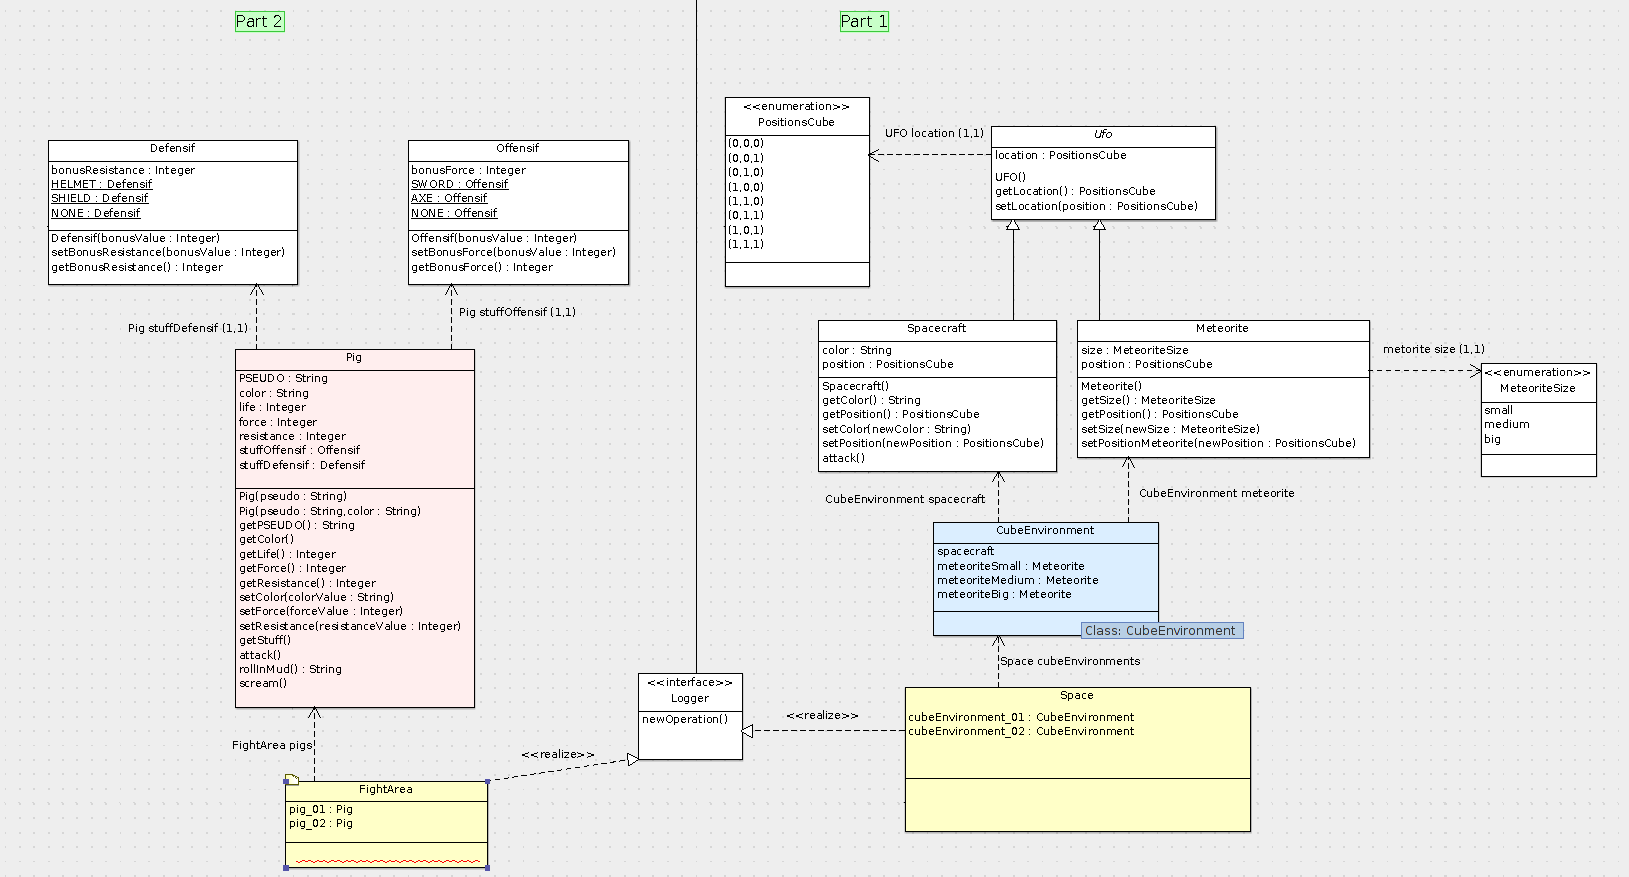
\includegraphics[width=450pt]{../../Images/UMLdiagramme.png}

Since you can't see anything on this screenshot, there bigger screenshots below.

Blue classes are abstract classes.\\
Green classes are interface.\\
Pink classes are enumeration.\\
Yellow classes are the two main classes from the 2 different parts of the game.\\

\begin{figure}
  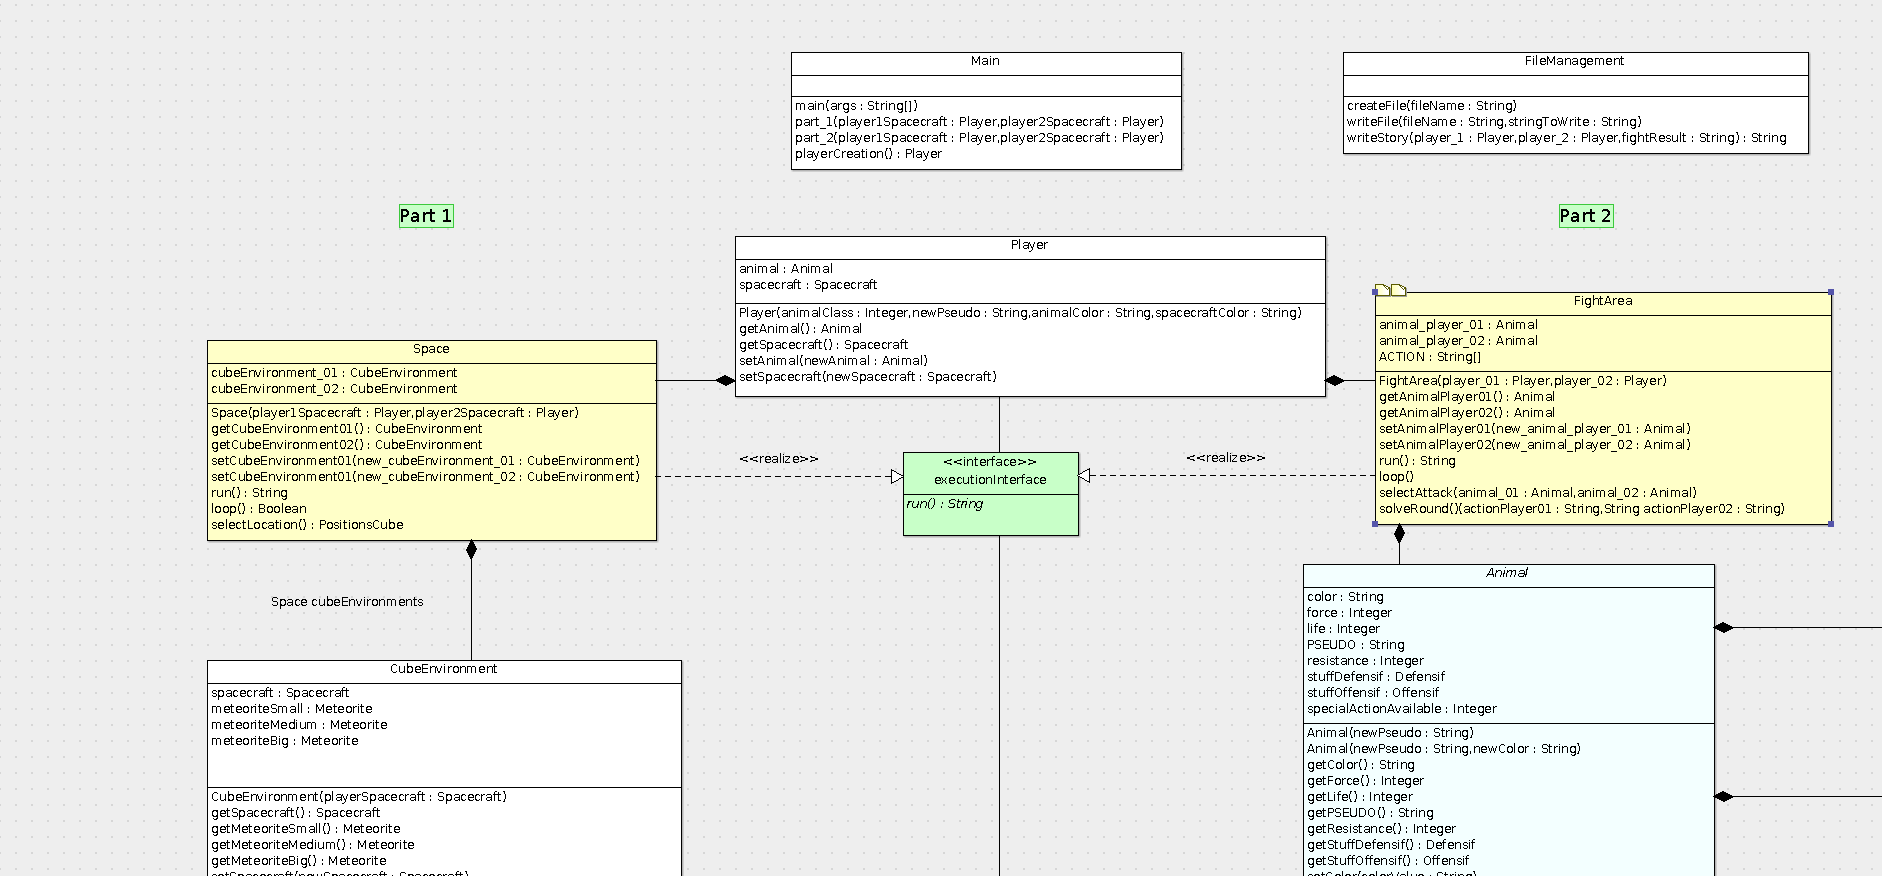
\includegraphics[width=450pt]{../../Images/1_1-2_1.png}
  \caption{\small left screenshot 1}
  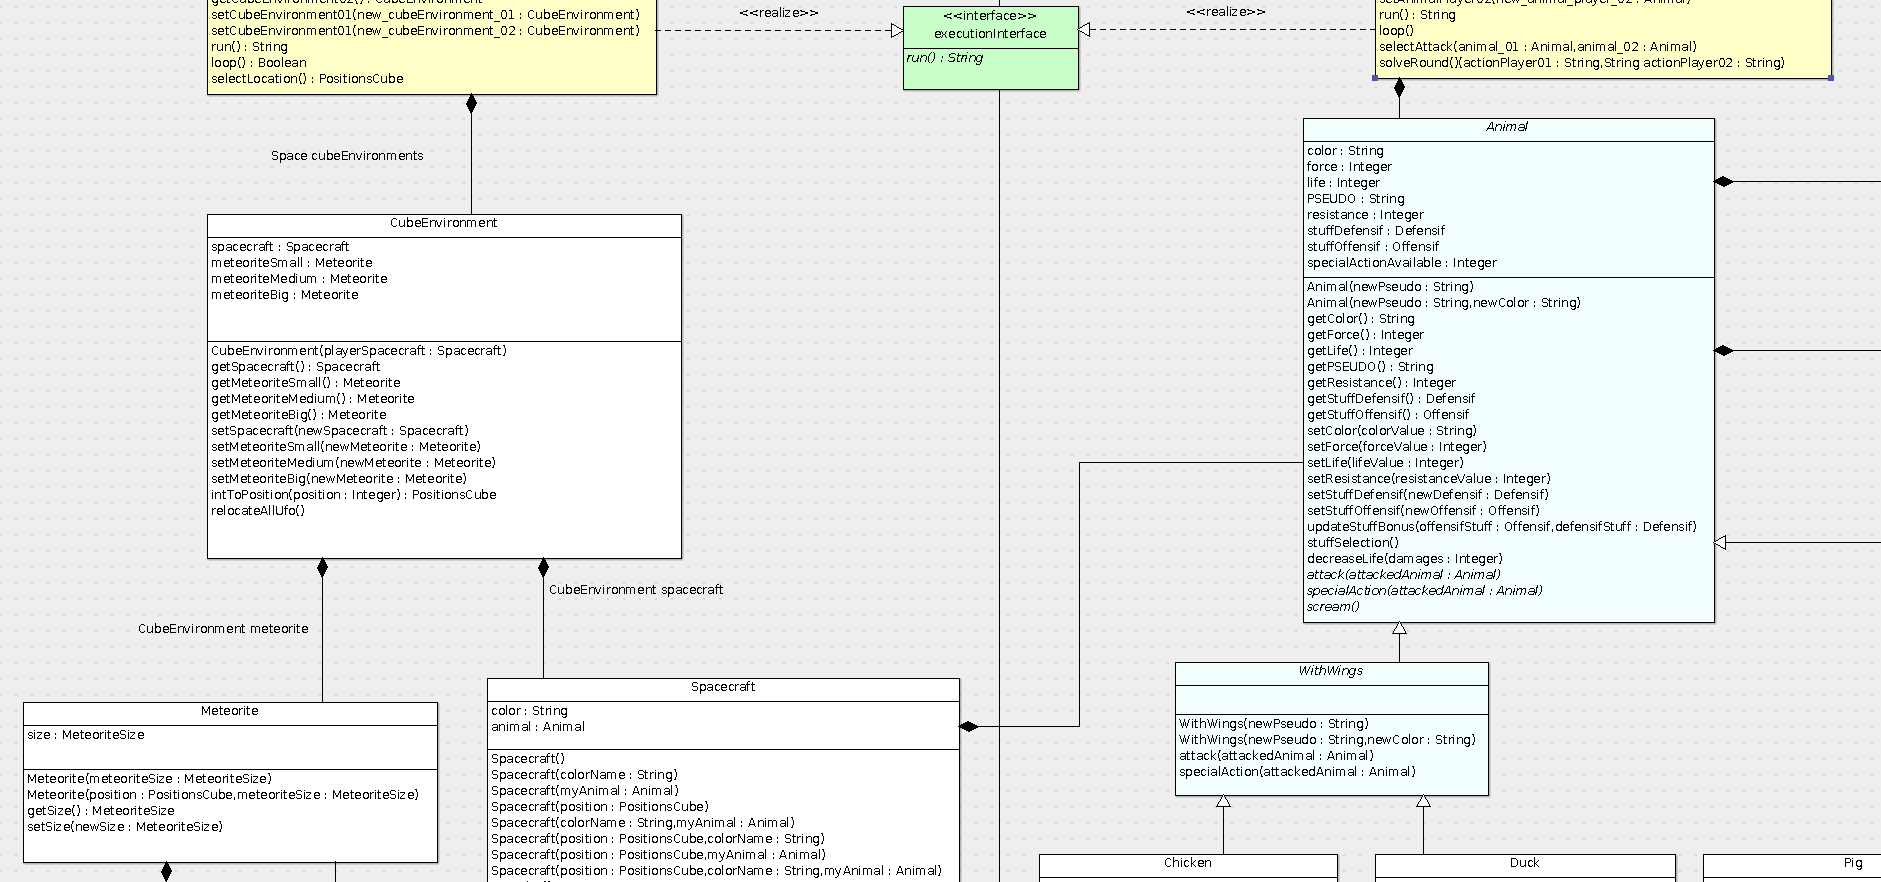
\includegraphics[width=450pt]{../../Images/1_1-1_2-2_2.png}
  \caption{\small left screenshot 2}
  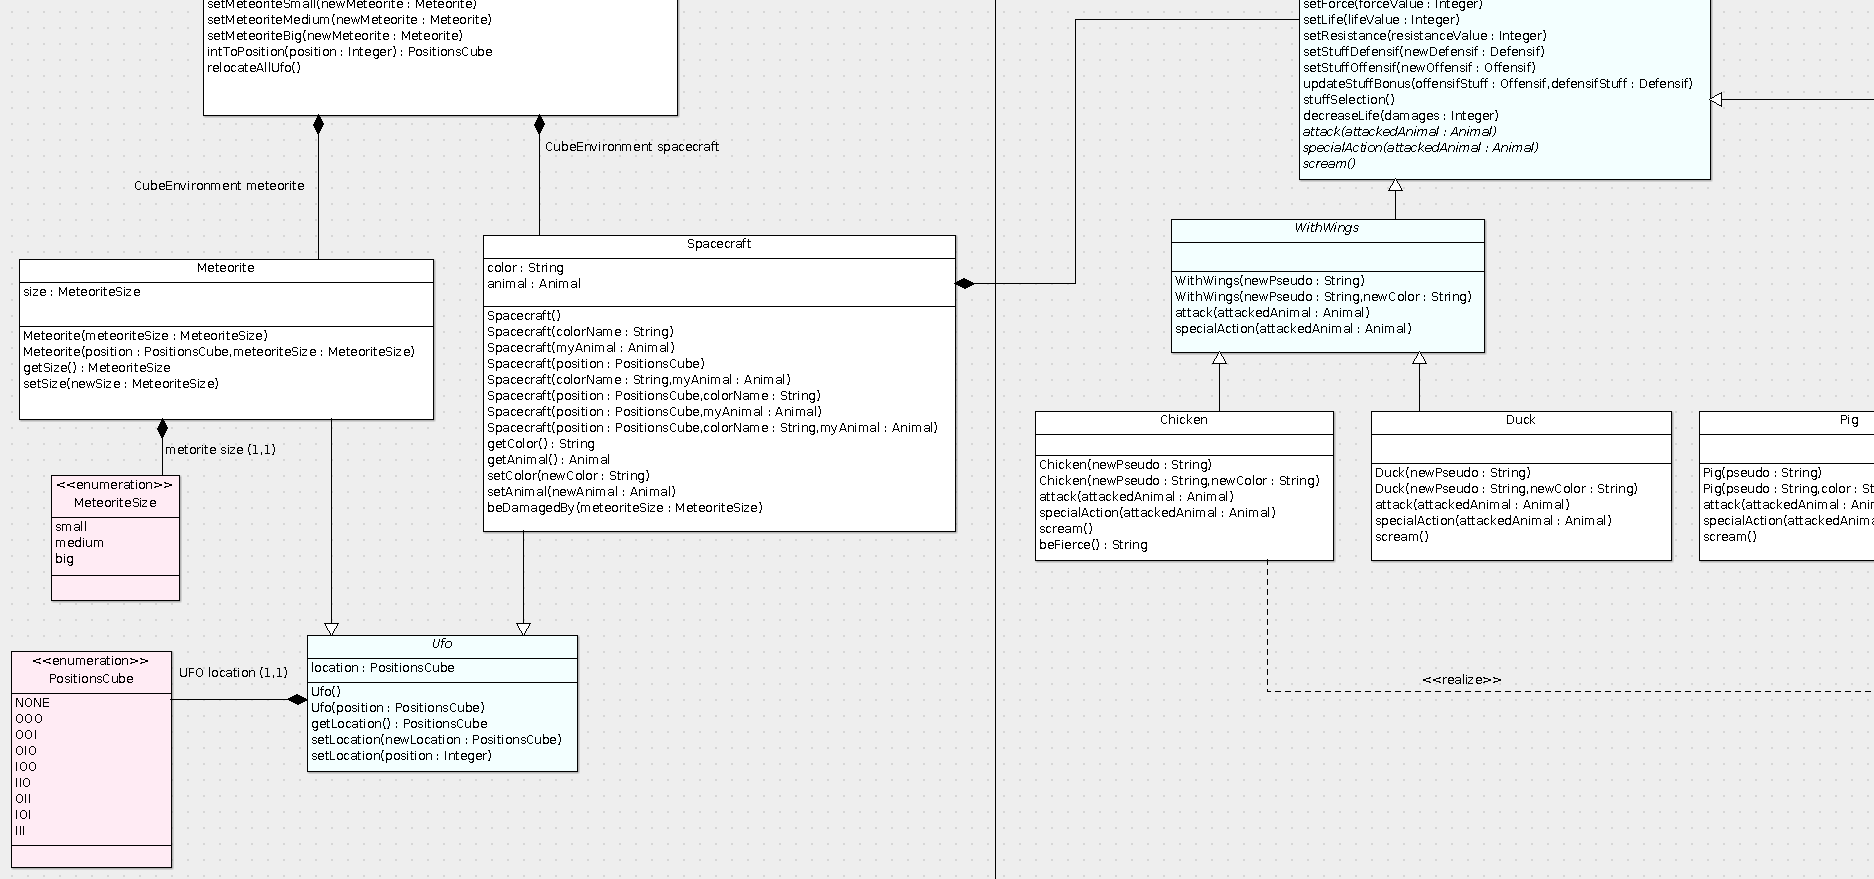
\includegraphics[width=450pt]{../../Images/1_2-2_3.png}
  \caption{\small left screenshot 3}
\end{figure}

\begin{figure}
  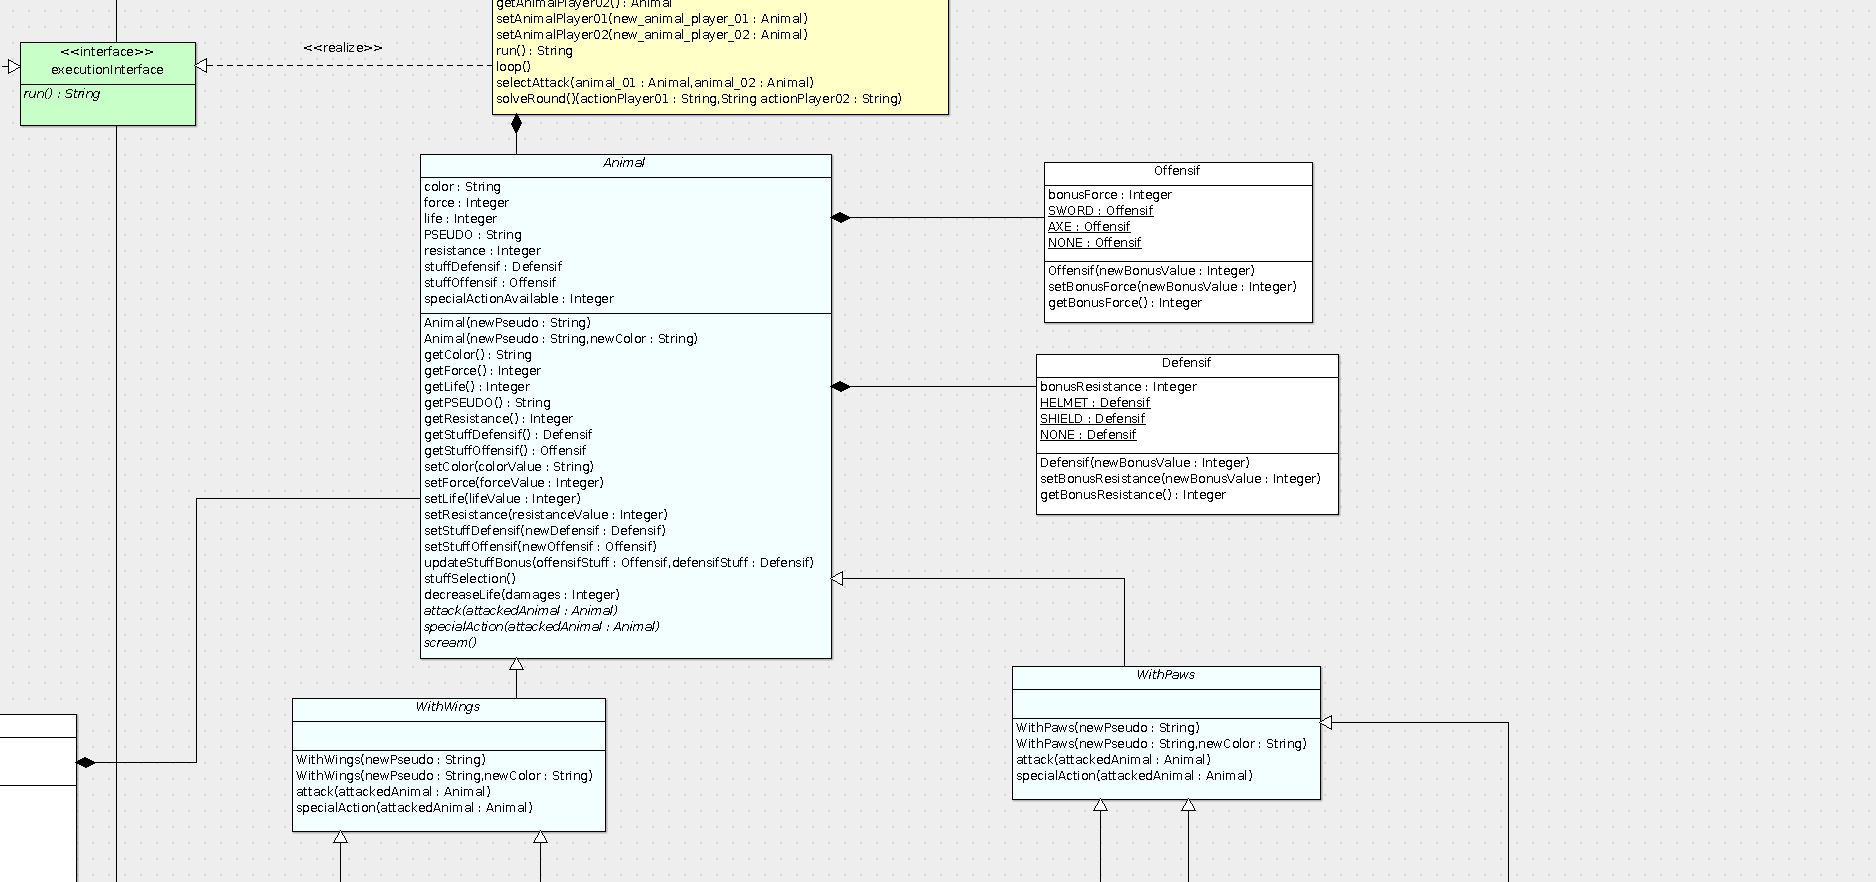
\includegraphics[width=450pt]{../../Images/2_2-3_2-3_3.png}
  \caption{\small right screenshot 1}
  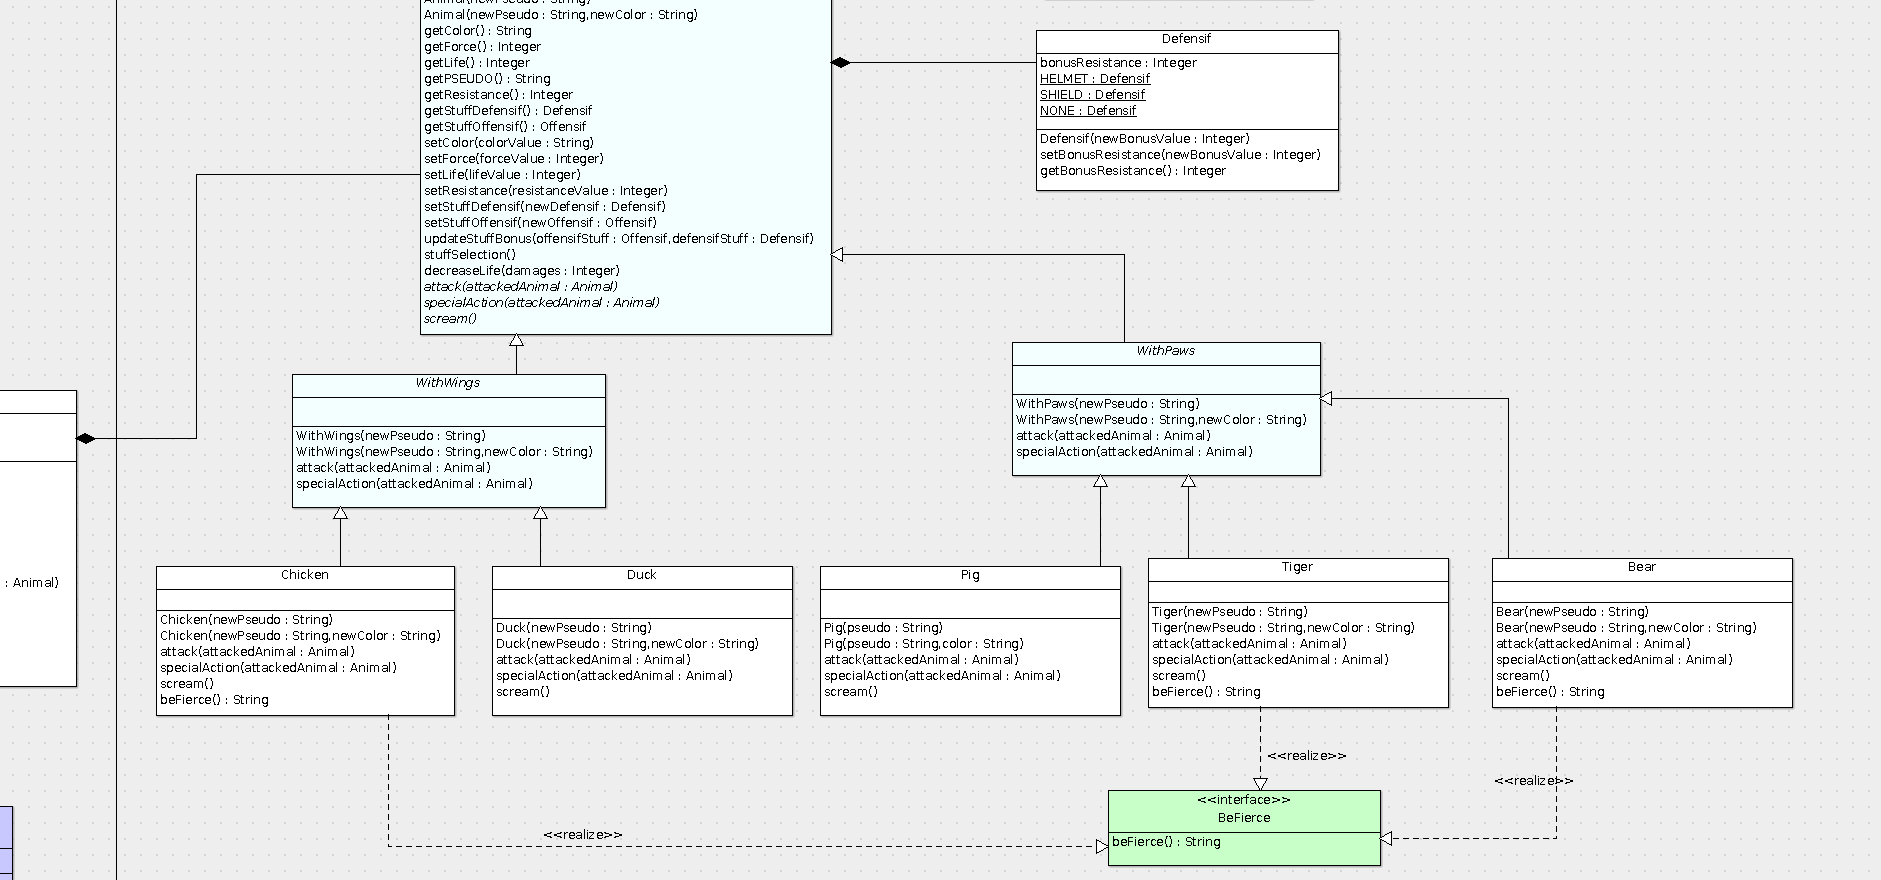
\includegraphics[width=450pt]{../../Images/2_3-3_3.png}
  \caption{\small right screenshot 2}
\end{figure}

\section{Technical part: class description}

<insert here: brief class description>

\subsection{Main}

This class contains the main functions:

\begin{itemize}
 \item main : main function that calls all the following functions.
 \item playerCreation : function that create the 2 players.
 \item part\_1 : function that runs game part 1.
 \item part\_2 : function that runs game part 2.
\end{itemize}


\subsection{FileManagement}

This class contains all useful functions to save the game story in a file. 
We chose to put them in a class in order not to overload the Main class.

\subsection{Player}

We created a Player class that keeps all information about each player. 
That is to say that a player contains a spacecraft and its animal.
It is from this class that we can access all information at any time and everywhere in our code.

\subsection{The 2 main classes of the game}

We created 1 class for each part of the game. 
It is from these 2 classes that each part is run.
They both implements the executionInterface interface.

\subsubsection{executionInterface interface:}

This interface has only one function: \textit{run()}. 
We decided to create this interface in order to create a name convention for the function which runs each part of the game.
By doing this, the Main class won't change, it will always call the \textit{run()} function of each class even if each class change.

\subsubsection{Space class:}

It is composed by 2 CubeEnvironments created thanks to the 2 Players.

\subsubsection{FightArea class:}

It is composed by 2 Animals created thanks to the 2 Players.


\subsection{Part1}

\subsubsection{CubeEnvironment class}

We thought the space environment in a particular way. 
Indeed, we assimilate it to 2 cubes, 1 for each player. That's why the Space class is composed of 2 CubeEnvironment.
Each cube is composed of a spacecraft and 3 meteorites. 
They can be located to 8 different positions that correspond to each corner of the cube.\\
\\
During the 1st part of the game, each player try to find the location of the other one's spacecraft.
Of course he has to avoid meteorites that decrease the life. 
Once one player find the other one, part 2 of the game is started.

\subsubsection{UFO class}

It is an abstract class. 
It was created in order to manage position of both meteorites en spacecrafts.
That's why Meteorite class and Spacecraft class both extends UFO abstract class.\\
\\
To manage location, an UFO has an attribute \textit{location}.
We also created function which make us be able to manage location.
Constructor was overloaded in order to create a UFO default position (000) or take the position in parameter.

\subsubsection{PositionsCube enumeration}

This enumeration enumerates all available positions in a cube. 
These positions match each corner of the cube.
They are coordinates.

\subsubsection{meteorites}

\subsubsection{MeteoriteSize}

This enumeration enumerates all existing meteorite size.

\subsubsection{spacecraft}


\subsection{Set the game}

\begin{itemize}
 \item set Player class for each player.
 \item set Space class with 2 CubeEnvironment (1 for each player). Each CubeEnvironment is set with 3 meteorites and 1 spacecraft.
 \item set FightArea class with 2 pigs. Each pig is initialized with stuff selected by the player.
\end{itemize}


\section{Encountered difficulties}

\subsection{Special action}

Special actions are very different. So we had to think our code so that it would be able to welcome each special action.
We had to modify our code.

\subsection{Exception}

We created an exception. We had difficultie because it was the first time and we didn't undertand exception very well.
We no longer do !


